\documentclass[10pt]{article}
\usepackage[utf8]{inputenc}
\usepackage[T1]{fontenc}
\usepackage{amsmath}
\usepackage{amsfonts}
\usepackage{amssymb}
\usepackage[version=4]{mhchem}
\usepackage{stmaryrd}
\usepackage{bbold}
\usepackage{graphicx}
\usepackage[export]{adjustbox}
\graphicspath{ {./images/} }
\usepackage{hyperref}
\usepackage[spanish]{babel}
\hypersetup{colorlinks=true, linkcolor=blue, filecolor=magenta, urlcolor=cyan,}

\title{El Algoritmo SWAG; un enfoque matemático que supera el aprendizaje profundo tradicional. Teoría e Implementación}


\author{Saeid Safaei ${ }^{1}$, Vahid Safaei $^{2}$, Solmazi Safaei $^{2}$, Zerotti Woods ${ }^{3}$,\\
Hamid R. Arabnia*$^{1}$, Juan B. Gutierrez*$^{1,3,4}$\\
$^{[1]}$Departamento de Ciencias de la Computación, Universidad de Georgia\\
$^{[2]}$Ingeniería Mecánica, Universidad de Yasouj\\
$^{[3]}$Departamento de Matemáticas, Universidad de Georgia\\
$^{[4]}$Instituto de Bioinformática, Universidad de Georgia\\
\{ssa, zerotti. woods 25 , hra, jgutierr\}@uga. edu\\
*Autores correspondientes conjuntos.}
\date{30 de noviembre de 2018}


\begin{document}
\maketitle
\begin{abstract}
El rendimiento de las redes neuronales artificiales (ANN) está influenciado por la inicialización del peso, la naturaleza de las funciones de activación y su arquitectura. Existe una amplia gama de funciones de activación que se utilizan tradicionalmente para entrenar una red neuronal, por ejemplo, sigmoid, tanh y Unidad lineal rectificada (ReLU). Una práctica muy extendida es utilizar el mismo tipo de función de activación en todas las neuronas de una capa determinada. En este manuscrito, presentamos un tipo de red neuronal en la que las funciones de activación en cada capa forman una base polinomial;
llamamos a este método SWAG por las iniciales de los apellidos de los autores. Probamos SWAG en tres funciones complejas altamente no lineales, así como en el conjunto de datos de escritura a mano MNIST. SWAG supera y converge más rápido que el rendimiento de última generación en redes neuronales totalmente conectadas.
\end{abstract}
\section{Introducción}

El aprendizaje profundo permite que los modelos computacionales que se componen de múltiples capas de procesamiento aprendan representaciones muy abstractas de datos [LBH15]. Ha habido informes de muchos éxitos
en el uso de redes neuronales profundas (DNN) en áreas como la visión artificial, el reconocimiento de voz, el procesamiento del lenguaje, el descubrimiento de fármacos, la genómica y muchas otras áreas. [JSA15]. Las DNN nos han permitido resolver problemas difíciles y han motivado un extenso trabajo para comprender sus propiedades teóricas [HDR18].
El proceso de cómo entrenar efectivamente un DNN es una tarea complicada y se ha demostrado que es un problema NP-Completo [BR89]. Características como la inicialización del peso, la naturaleza de las funciones de activación y la arquitectura de la red pueden afectar el proceso de entrenamiento de una red
neuronal [Sch15] [HDR18] [RZL18]. En particular, algunas opciones de funciones de activación o arquitecturas de red pueden causar pérdida de información o pueden aumentar la cantidad de tiempo necesario para
entrenar un DNN [HDR18][ZL18][CLP16][LTR17]. La cuestión de cómo encontrar de manera efectiva el mejor conjunto de funciones de activación no lineal es un desafío [CLP16]. Algunas de las funciones de activación no lineales más conocidas son:
$$
\begin{aligned}
\operatorname{sigmoid}(x) &=1 /\left(1+e^{-X}\right) \\
\tanh (x) &=\left(1-e^{-2 X}\right) /\left(1+e^{-2 X}\right) \\
\operatorname{ReLU}(x) &=\max (x ; 0)
\end{aligned}
$$
La función de activación en la ecuación (3) Unidad lineal rectificada (ReLU), es la función de activación más popular y ampliamente utilizada; y aunque se han introducido algunas funciones de activación diseñadas a mano para reemplazar a ReLU, ninguna ha ganado la popularidad que tiene ReLu [MHN13][CUH15] [KUMH17] [HSM+00] [JKL+09] [NH10]. Las funciones de activación no lineales entrenables han sido propuestas por [CLP16], [TGY04]. Chung et al.[CLP16] usó una aproximación en serie de Taylor desigmoideo,bronceado, yReLUcomo punto de inicialización de sus funciones de activación, y entrenó los coeficientes de la aproximación de la serie de Taylor para optimizar el entrenamiento. Esta implementación utilizó la misma función polinomial en cada neurona de una capa determinada. Los resultados fueron comparables al estado del arte. En este manuscrito, presentamos un tipo de red neuronal en la que las funciones de activación en cada capa forman una base polinomial, es decir, grupos de neuronas se asignan a monomios únicos en una capa dada. También proponemos una nueva arquitectura en la que concatenamos verticalmente muchas capas completamente conectadas para formar una capa que hace que el cálculo sea más eficiente. No entrenamos
funciones de activación. Nuestras funciones de activación son fijas y forman una base polinomial. La estructura de las capas ocultas sigue el patrón de: (i) una capa con polinomios como funciones de activación, y (ii) una capa con una función de activación lineal. El resto de este manuscrito está organizado de la siguiente manera: la Sección 2 describe los fundamentos matemáticos y la arquitectura de SWAG, la Sección 3 describe los experimentos que se
realizaron y la Sección 4 es una discusión de los resultados y el trabajo futuro.

\section{Métodos}

\subsection{Representación de funciones con base}
Supongamos que tenemos un conjunto de datos $\left\{\mathbf{x}_{j}\right\}$ para $1 \leq j \leq n$ y etiquetas $\left\{\mathbf{y}_{j}\right\}$ que corresponden con nuestro conjunto de datos. Nos gustaría encontrar una función $f(x)$ tal que $f\left(x_{j}\right)=y_{j}$ para todo $1 \leq j \leq n$. El teorema de aproximación de Stone-Weierstrass establece que cualquier función continua de valor real en un conjunto compacto puede aproximarse uniformemente mediante un polinomio. Formalmente:

Teorema 2.1 (Teorema de aproximación de Stone-Weierstrass). Suponga que $f$ es una función continua de valor real definida en cualquier subconjunto cerrado y acotado $X \in \mathbb{R}^{m}$ para cualquier $m \in \mathbb{N}$. Para todo $\epsilon>0$, existe un polinomio $p\left(x_{1}, x_{2}, \ldots, x_{m}\right)$ tal que $\left|f\left(x_{1}, x_{2}, \ldots, x_{m}\right)-p\left(x_{1}, x_{2}, \ldots, x_{m}\right)\right|<\epsilon$ para cualquier $\left(x_{1}, x_{2}, \ldots, x_{m}\right) \in X$

La simplicidad de los sistemas polinómicos los hace muy atractivos desde el punto de vista analítico y computacional. Son fáciles de formar y tienen propiedades bien entendidas. El uso de polinomios de un grado dado como funciones de activación para todas las neuronas en una sola capa parece
desaconsejarse matemáticamente en los entornos de redes neuronales tradicionales porque no son aproximadores universales. En particular, Leshnoy otros. (1993) [LLPS93] demostró el siguiente teorema:

Teorema 2.2. Sea $M$ el conjunto de funciones que son $L_{l o c}^{\infty}(\mathbb{R})$ with con la propiedad de que el cierre de la conjunto de puntos de discontinuidad de cualquier función en $M$tiene medida de Lebesgue cero. Sea $\sigma \in M$. Entonces para una $x \in \mathbb{R}^{n}$,
$$\operatorname{span}\left\{\sigma\{w \cdot x+\Theta\}: w \in \mathbb{R}^{n}, \Theta \in \mathbb{R}\right\}$$ es denso en $\mathbb{C}\left(\mathbb{R}^{n}\right)$ si y solo si $\sigma$ no es un polinomio algebraico (a.e.)
Este teorema implica que las redes neuronales feedforward totalmente conectadas con un número suficiente de neuronas son aproximadores universales si y solo si las funciones de activación no son polinomios. Observamos que en esta configuración tradicional se supone que la función de activación es la misma para cada neurona en una capa determinada. Ahora damos la siguiente extensión del teorema de aproximación de Stone-Weierstrass

Corolario 2.3. Sea $\sigma_{p}=\frac{x^{p}}{p !}$ for $0 \leq p<\infty$. Después
$$
\operatorname{span}\left\{\sigma_{p}\{w \cdot x+\Theta\}: w \in \mathbb{R}^{n}, \Theta \in \mathbb{R}\right\}
$$es denso en $\mathbb{C}\left(X^{n}\right)$ donde $X^{n} \in \mathbb{R}^{n}$ es un conjunto compacto.

Prueba.Ten en cuenta que $\left\{\sigma_{p}\right\}_{p=0}^{\infty}$ es una base para el espacio vectorial de polinomios sobre $\mathbb{R}$. Así que ya que nosotros sabemos que los polinomios son densos en $\mathbb{C}\left(X^{n}\right)$ por el teorema de aproximación de Stone-Weierstrass, el resultado es el siguiente.

Este corolario implica que si permitimos un conjunto diverso de funciones de activación polinómicas en una capa en particular, aún tendremos el resultado de las capacidades de aproximación universal de las redes neuronales de avance. Usando el mismo marco que Leshnoy otros. (1993) [LLPS93], en el que se supuso que la salida estaba en $\mathbb{R}^{n}$, se puede obtener fácilmente una extensión a dimensiones más altas redefiniendo $\sigma_{p}\{w\}$ como una operación puntual que toma cada elemento de $w$ y lo eleva a la $p^{\text {th }}$ potencia, e.g. dado $w=[2,3]$, entonces $\sigma_{4}\{w\}=\left[2^{4}, 3^{4}\right]$.

\subsection{Arquitectura del Algoritmo SWAG}
Dejar $x_{j} \in \mathbb{R}^{d}$ ser un punto de datos en nuestro conjunto de datos $\left\{x_{j}\right\}_{j=1}^{n}$.

0 Normalice los datos para que estén en el intervalo $[0,1]$.

1 Cree la primera capa polinomial de la siguiente manera:

1.1 Elegir un $k$ para el número de términos polinómicos utilizados ($k$ es un hiperparámetro del modelo).

$1.2$ Elegir $l$ por el número de neuronas que corresponden a cada monomio del $1^{\text {st }}$ capa ( $l$ es un hiperparámetro).

1.3 Crear $k$ capas totalmente conectadas con $l$ neuronas en cada capa, todas con $x_{j}$ como sus entradas.

1.3.1 El $p^{\text {th }}$ capa completamente conectada $1 \leq p \leq k$ es definido por $\sigma_{p}\{W x+b\}$ for $W \in$ $l \times d, b \in \mathbb{R}^{l}$, and $\sigma_{p}$ cpmo se define arriba.

1.3.2 La inicialización de los pesos es aleatoria y extraída de $\mathcal{N}(0,1)$,como una distribución gaussiana con media 0 y desviación típica 1. 1.4 Concatenar verticalmente loskcapas para formar un vector de longitud $l \cdot k$

2 Cree una capa con una función de activación lineal. Esto se considera la segunda capa de SWAG.

3 Para agregar una tercera y cuarta capa, repita la estructura de las 2 capas anteriores con la entrada de la tercera capa como la salida de la segunda capa. Si se agrega una tercera y una cuarta capa,la primera dimensión de la matriz utilizada en la segunda capa es un hiperparámetro del modelo..

4 Continúe agregando capas en este patrón según lo desee.

5 La matriz utilizada para la capa final de activación lineal tendrá como primera dimensión la dimensión del vector de salida.

Figura 1 es un diagrama de un ejemplo de SWAG que usa dos capas y la figura 3 es un diagrama de un ejemplo de SWAG con cuatro capas.

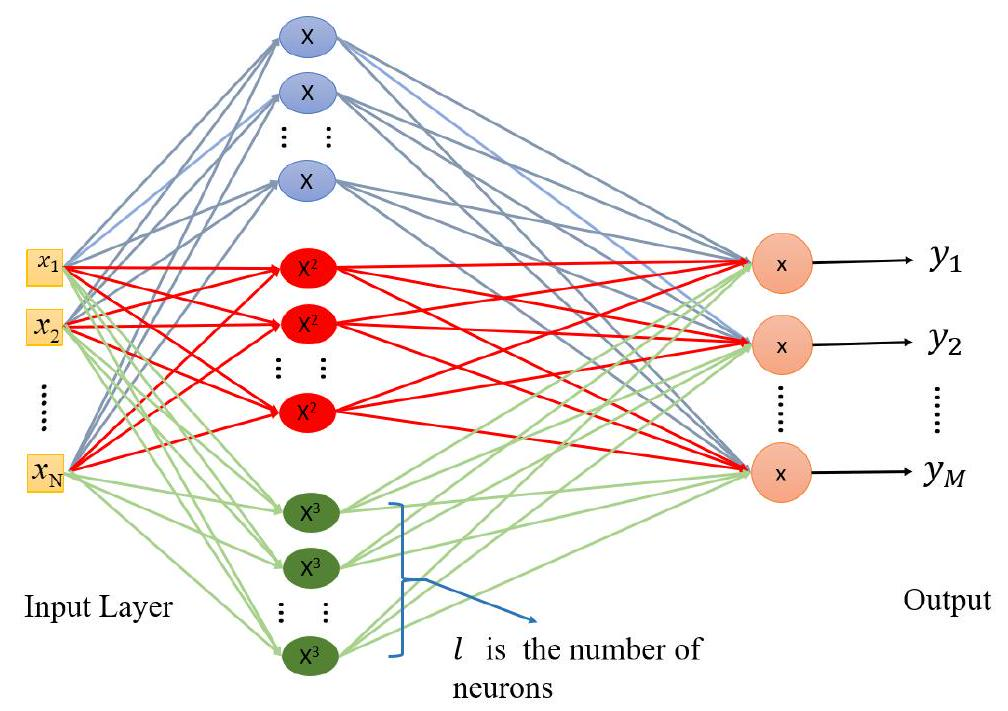
\includegraphics[max width=\textwidth]{2022_09_28_0067ec14010042dbf918g-04}

Figura 1: Implementación de la arquitectura SWAG con tres grupos de monomios de potencias 1 a 3, y dos capas

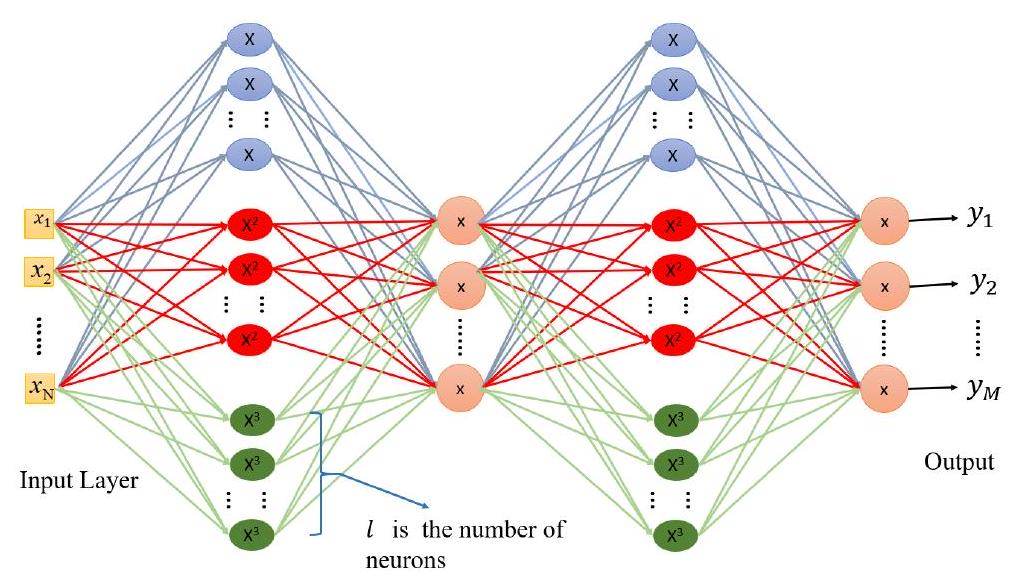
\includegraphics[max width=\textwidth]{2022_09_28_0067ec14010042dbf918g-05}

Figura 2: Implementación de la arquitectura SWAG con tres grupos de monomios de potencias 1 a 3, y cuatro capas

\section{Resultados}
\subsection{Representación de funciones no lineales}
Para probar nuestro modelo, generamos un conjunto de datos aleatorios $X_{\text {train }}=\left\{x_{j}\right\}_{j=1}^{1000}$, con $x_{j} \in(0,1)$ como vector de entrenamiento $X_{\text {test }}=\left\{x_{k}\right\}_{k=1}^{200}$, con $x_{k} \in(0,1)$ como vector para la prueba. Seleccionamos
tres funciones para las cuales los DNN tradicionales no convergen en absoluto, o requieren un número de épocas de órdenes de magnitud mayor que SWAG para converger.
$$
\begin{gathered}
F_{1}=\frac{1}{2} x^{2}-5\left(\frac{1}{1+e^{x}}\right) \\
F_{2}=6 x^{5}-3\left(\frac{1}{1+e^{x}}\right)+e^{x}-9 \log _{10}(x) \\
F_{3}=22 x^{20}-\frac{1}{1+e^{x}}+2 e^{x}+5 \log _{10}(x) \\
1 \leq i \leq 3 \quad Y_{i_{\text {train }}}=F_{i}\left(X_{\text {train }}\right) \quad Y_{i_{\text {test }}}=F_{i}\left(X_{\text {test }}\right)
\end{gathered}
$$
Entrenamos 5 DNNs tradicionales de varias arquitecturas (código en apéndice). También capacitamos a SWAG, conyo=50,k=8, y usamos 4 capas. La primera dimensión de la segunda capa en esta implementación de
SWAG fue 50. Usamos la función de pérdida cuadrática media estándar con el optimizador de Adam para probar la precisión del modelo [KB14].

Realizamos un primer experimento para, $F_{1}$, como se muestra en la Figura 3. SWAG es el único modelo en el que la función de costo converge a cero después de 50 épocas de entrenamiento en $F_{1}$.También notamos que la Figura 4 da una representación visual de cómo las diferentes arquitecturas reconstruyeron $F_{1}$.

Realizamos un segundo experimento con $X_{\text {train }}=\{0.01,0.02,0.03, \ldots, 1\}$ y $X_{\text {test }}=\{0.015,0.025,0.035 \ldots, 0.985\}$.Esto permite que los conjuntos de prueba y entrenamiento tengan casi la misma cantidad de puntos.
$$
1 \leq i \leq 3 \quad Y_{i_{\text {train }}}=F_{i}\left(x_{\text {train }}\right) \quad Y_{1_{\text {test }}}=F_{1}\left(x_{\text {test }}\right)
$$
Repetimos el proceso del primer experimento para entrenar y probar los distintos modelos. Los resultados de los dos experimentos se encuentran en las Figuras 5-14 del apéndice.\\
